\chapter{Aplikacje klienckie}

\section*{Aplikacja Android}

Opis Androida, screenshoty


\section*{Aplikacja iOS}
Aplikacja przeznaczona jest na urządzenia z systemem operacyjnym iOS od wersji 10.0. 
Nie wspiera ona wcześniejszych wersji ze względu na nowe funkcje, które Apple wprowadziło wraz z pojawieniem się iOS 10.0 (m.in. klasa UNUserNotificationCenter). Jednak jak wynika z wykresu niżej (numer rysunku) 92\% wszystkich obecnych użytkowników tego systemu jest w stanie zainstalować aplikację a liczba ta stale rośnie. Aplikacja wykonana została wspierając zarówno telefony komórkowe iPhone jak i tablety iPad. 
\begin{figure}[h]
	\centering
	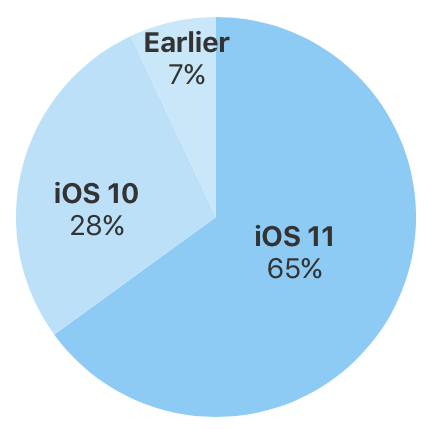
\includegraphics[width=6cm]{iOSstat}
	\caption{Udziały wersji systemu iOS w rynku}
\end{figure}
Napisana jest w stosunkowo nowym języku Swift (został zaprezentowany przez Apple w 2014r na konferencji WWDC) w oparciu o architekturę MVC (Model-View-Controller) wykorzystując przy programowanie reaktywne i funkcjonalne. 
Programowanie reaktywne zrealizowano przy pomocy biblioteki RxSwift. Wykorzystano je m.in w celu wznowienia streamu obrazu z kamery w momencie przejścia aplikacji z trybu Background do trybu Foreground. Oznacza to, że w momencie wyjścia z aplikacji ale pozostawiając ja działającą w tle i po chwili uruchomienia jej ponownie traciliśmy obraz Video, ze względu na politykę bezpieczeństwa Apple, która nie zezwala aby aplikacje pobierały dane przez dłuższy okres czasu kiedy aplikacja pracuje w tle. Dzięki programowaniu reaktywnemu problem ten został rozwiązany co prezentuje poniższy kod:
\begin{verbatim}
let appDelegate = UIApplication.shared.delegate as! AppDelegate
        appDelegate.inBackground.asObservable().subscribe(onNext: { (value) in
            if let streamView = self.streamView {
                if let player = self.currentPlayer {
                    if value == false {
                        self.streamVideoFrom(urlString: self.currentUrlString!)
                        print("Enter foreground")
                    } else {
                        print("Enter background")
                        streamView.layer.sublayers?.forEach({ (layer) in
                            layer.removeFromSuperlayer()
                        })
                    }
                }
            }
        }).disposed(by: disposeBag)
\end{verbatim}
Zmienna inBackground ustawiana jest oddzielnej klasie AppDelegate na wartość true kiedy aplikacja przechodzi w tryb background i na wartość false w przeciwnym wypadku. Kod powyżej uruchamia się za każdym razem przy zmianie tej wartości i uruchamia stream po każdym ponownym uruchomieniu programu.
Programowanie funkcjonalne natomiast wykorzystane jest w miejscach gdzie konieczne jest przekształcenie danych do innej postaci:
\begin{verbatim}
lastNotification = notifications.array.sorted(by: { (n1, n2) -> Bool in
	n1.date > n2.date 
}).filter({ (notif) -> Bool in return notif.type == "PIRSensor"}).first
\end{verbatim}
Na tablicy z notyfikacjami zastosowano szereg funkcji: posortowano je malejąco według daty, przefiltrowano w taki sposób aby wybrać tylko te o typie 'PIRSensor' czyli tylko te pochodzące z czujnika ruchu. Na sam koniec wybrano tylko jeden pierwszy element z wybranych i wynik wpisano do zmiennej lastNotification.

Strukture kodu(rys. 5.2) podzielono na kilka osobnych logicznych części. Folder Firebase zawiera model bazy danych czujników, które trzymane są na serwerach Firebase. W folderze GuardManager znajdują sie elementy odpowiedzialne za komunikację REST-ową z serwerem Django i również modele bazy danych znajdującej się na naszym serwerze. Folder Views jest zbiorem widoków, które wczytywane są w zależności, w której sekcji się znajdujemy (opis sekcji niżej). ViewController.swift jest głównym kontrolerem zarządzającym widokami i modelami. W folderze GuardianAppTests napisane zostały testy jednostkowe, które sprawdzają poprawność przekształcania danych typu JSON do obiektów zdefiniowanych w folderze GuardManager/Models. Klasy, których nazwy kończą się na Manager oznaczają obiekty typu Singleton. Celem takiego wzorca jest zapewnienie istnienia tylko jednej instancji w całej aplikacji i globalnego dostępu do tego obiektu. GuardManager, który odpowiada za pobieranie danych z bazy danych - taki obiekt nie powinien być utworzony więcej niż jeden raz, gdyż wszystkie klasy, które z niego korzystają nie potrzebują kolejnych instancji tej klasy. W ten sposób zapewniamy, że zawsze odwołujemy się do tego samego obiektu.

\begin{figure}[h]
	\centering
	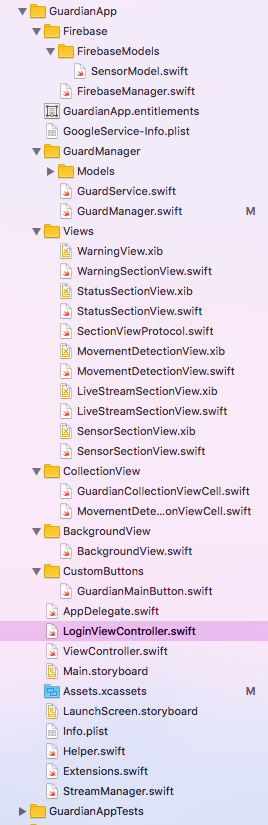
\includegraphics[width=4cm]{iOSstructure}
	\caption{Struktura aplikacji}
\end{figure}


Instalacja zewnętrznych bibliotek odbywa się za pomocą CocoaPods. Jest to menadżer zależności dzięki któremu szybko możemy wyszukać i zainstalować wymagane oprogramowanie. Wszystkie użyte zależności przedstawia poniższy listing: 

\begin{verbatim}
  pod 'Moya'
  pod 'MBProgressHUD', '~> 1.0'
  pod 'RxSwift',    '~> 4.0'
  pod 'RxCocoa',    '~> 4.0'
  pod 'IHKeyboardAvoiding'
  pod 'Moya-SwiftyJSONMapper'
  pod 'Firebase/Core'
  pod 'Firebase/Messaging'
  pod 'Firebase/Auth'
  pod 'Firebase/Database'
  pod 'M13ProgressSuite'
\end{verbatim}
Moya używana jest do asynchronicznej REST-owej komunikacji z serwerem Django. SwiftyJSONMapper przydatna okazuje się do przekształcenia odpowiedzi serwera w postaci JSON'a do wcześniej zdefiniowanego modelu. MBProgressHUD umożliwia wyświetlanie ekranu ładowania danych podczas pobierania informacji z serwera. RxSwift i RxCocoa to biblioteki do programowania reaktywnego. Moduły Firebas/Core itp. służą do komunikacji z serwerami Firebase. Ostatni 'pod M13ProgressSuite' służy do rysowania wykresów i animowanych elementów graficznych w systemie iOS.

Po uruchomieniu aplikacji pierwszym widokiem jest ekran logowania i rejestracji użytkowników(rys 5.2). 
\begin{figure}[h]
	\centering
	
\includegraphics[width=5cm]{login.png}
	\caption{Ekran logowania}
\end{figure}
Po prawidłowej autoryzacji danych użytkownika wprowadzonych podczas logowania ukaże się nam główny widok aplikacji. W górnej części mamy do wyboru 5 sekcji:
sekcja czujników, sekcja historii notyfikacji, sekcja zagrożeń przy wykryciu ruchu, sekcja streamu na żywo, sekcja ustawień. Wszystkie te sekcje dotyczą konkretnego urządzenia wybranego w pasku na dole ekranu. Przy pierwszym uruchomieniu nie będziemy posiadali żadnych urządzeń przypisanych do naszego konta użytkownika. Aby dodać pierwsze i kolejne stacje, od których chcemy otrzymywać notyfikacje o zagrożeniach a także śledzić i monitorować informacje z czujników należy wybrać przycisk "New" z plusikiem w dolnej części ekranu. Pojawi się okno z prośbą o wpisanie numeru identyfikującego jednoznacznie urządzenie. Po chwili dodany Guard będzie widoczny w na liście.
\paragraph{Sekcja czujników:}
Jest to jedna z najważniejszych sekcji aplikacji (rys 5.3).  Otrzymuje ona dane z czujników w czasie rzeczywistym i prezentuje je użytkownikowi.  W zależności od koloru prezentowanej wartości z czujnika użytkownik analizuje zagrożenie. Kolor zielony reprezentuje bezpieczne i prawidłowe odczyty na czujnikach, kolor pomarańczowy średnie, kolor czerwony reprezentuje bardzo wysoki poziom niebezpieczeństwa. Implementacja tej funkcjonalności zrealizowana została przy pomocy modelu HSV a nie RGB, dzięki temu zmieniając parametr Hue zmieniamy barwę przy stałym nasyceniu i jasności. Wartość tego parametru równa 120\textdegree{} odpowiada kolorowi zielonemu, kolor czerwony to 0\textdegree{}. Przekształcając wartość otrzymaną z czujników, która jest z zakresu [0-1] na wartość z przedziału [120-0] otrzymano wyżej wspomniany efekt. 
Poniżej przedstawiono fragment konwersji danych z czujników na kolor w modelu HSV, gdzie zmienna sensors[0] reprezentuje czujnik LPG.
\begin{verbatim}
UIColor(hue: CGFloat(0.33 - (sensors[0].value * 0.33)),
saturation: 1, brightness: 1, alpha: 1)
\end{verbatim}
\begin{figure}[h]
	\centering
	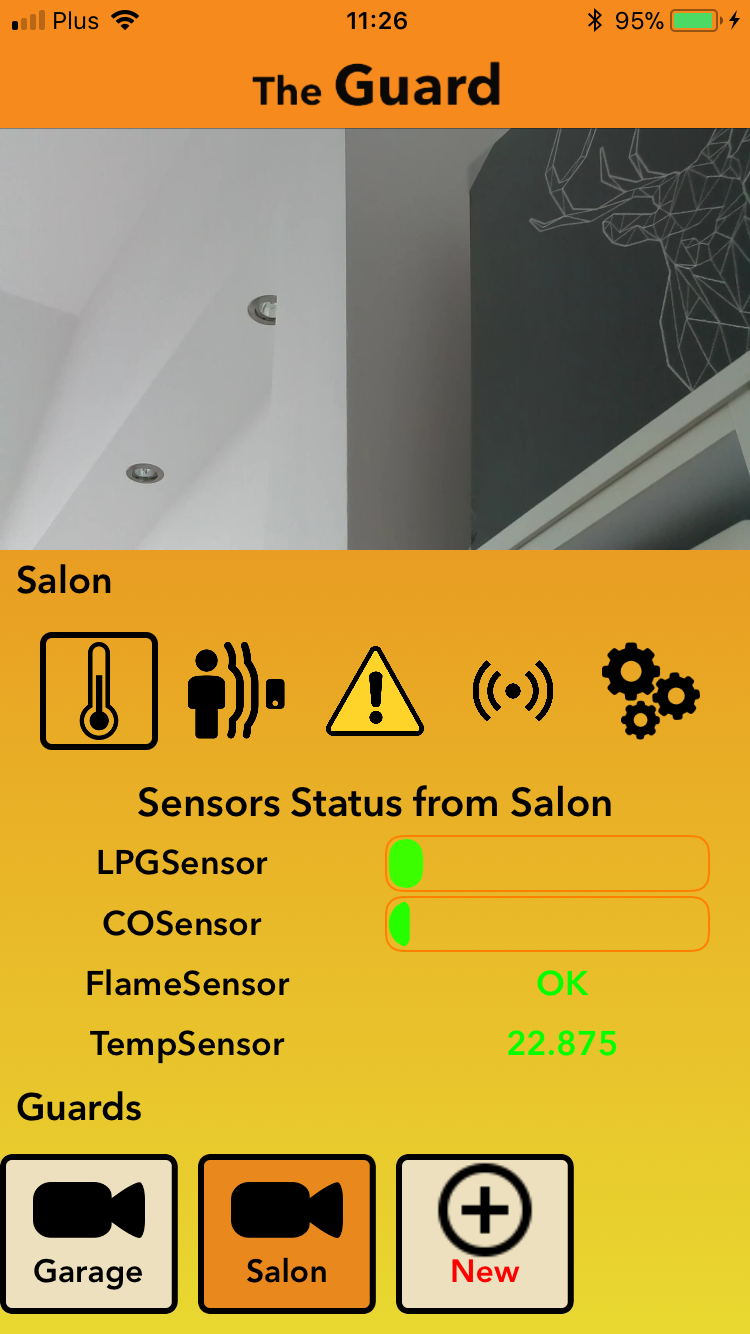
\includegraphics[width=5cm]{sensors.png}
	\caption{Sekcja czujników}
\end{figure}
\paragraph{Sekcja historii notyfikacji:}
W tej sekcji użytkownik ma dostęp do historii zdarzeń w systemie (rys 5.4). Po zaznaczeniu interesującego nas daty reprezentującej moment wystąpienia zagrożenia i wybranu przycisku 'preview' prezentowana jest informacja o miejscu niebezpieczeństwa i jego rodzaju.
\begin{figure}[h]
\centering
\begin{minipage}{.4\linewidth}
    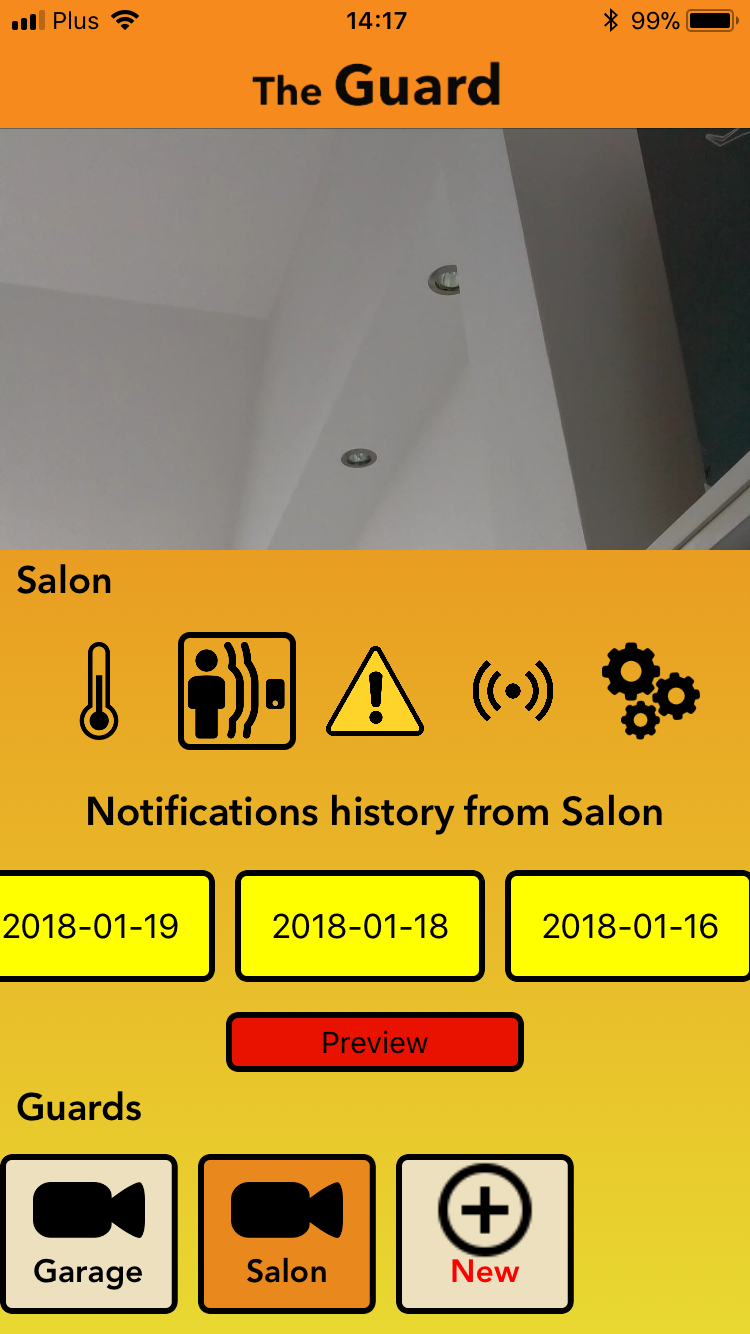
\includegraphics[width=\linewidth]{history.png}
    \caption{Sekcja historii notyfikacji}
    \label{img1}
\end{minipage}
\hspace{.05\linewidth}
\begin{minipage}{.4\linewidth}
    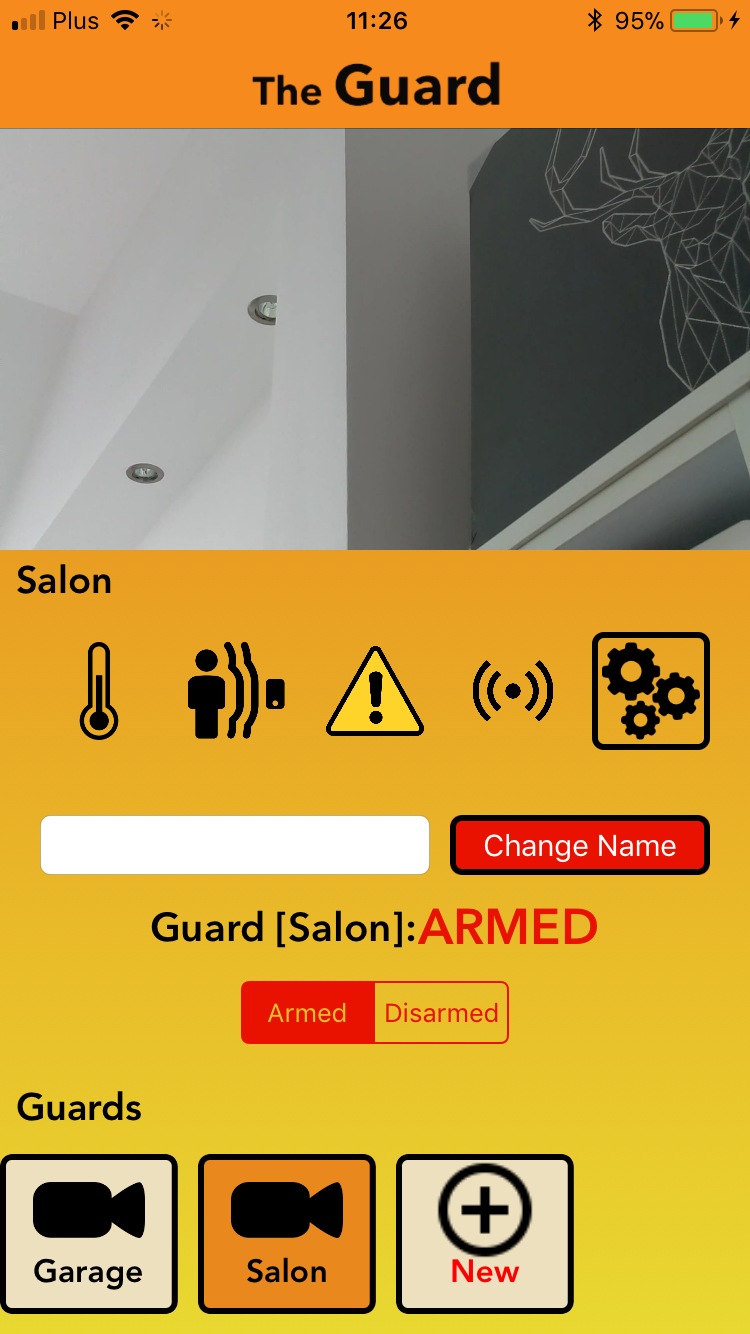
\includegraphics[width=\linewidth]{settings.png}
    \caption{Sekcja ustawień}
    \label{img2}
\end{minipage}
\end{figure} 
\paragraph{Sekcja ustawień:}
Ustawienia dotyczące zaznaczonego na dole ekranu urządzenia (rys 5.5). Użytkownik ma możliwość zmiany nazwy urządzenia, które zazwyczaj reprezentuje miejsce, w którym znajduje się stacja pomiarowa. Istnieje również możliwość uzbrojenia i wyłączenia konkretnego czujnika. Sprowadza się to do tego, że w przypadku zaznaczenia opcji "Disarmed" użytkownik nie będzie otrzymywał kolejnych notyfikacji o zagrożeniach. Opcja ta może okazać się przydatna w momencie uszkodzenia któregoś z modułów i tym samym błednych danych wysyłanych z czujników.
Przeprowadzono kilka testów aplikacji pod pełnym obciążeniem za pomocą programu Instruments. Szczególnie interesująco przedstawia się zużycie sieci podczas streamu obrazu. Widać, że w ciągu jednej minuty pobrano 6,61MB a wysłano jedynie 24,11Kb. Obraz pobierany jest tylko wtedy kiedy aplikacja jest aktywna. Nie musimy obawiać się, że stream jest aktywny, kiedy nie korzystamy z programu. W ciągu godziny działania aplikacji pobierze ona około 400MB danych.
\begin{figure}[h]
	\centering
	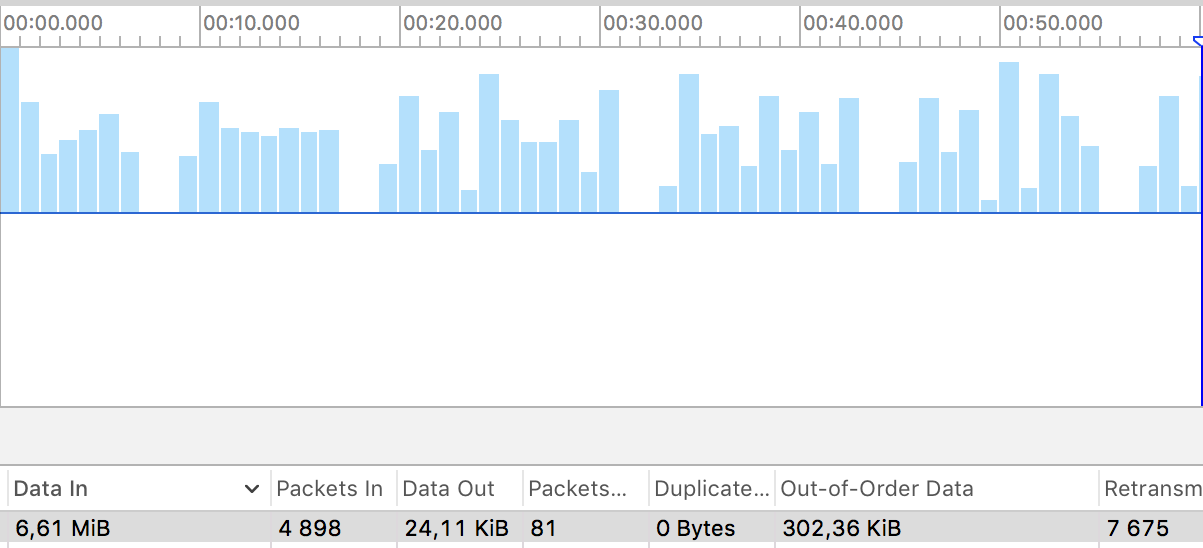
\includegraphics[width=10cm]{networkUsage}
	\caption{Zużycie sieci podczas streamu}
\end{figure}
Przeprowadzono także test na zużycie pamięci RAM i zużycia procesora. Te jednak są niewielkie i wynoszą odpowiednio 25MB pamięci RAM i średnio 1 procent zużycia procesora.
Testy przeprowadzono na iPhonie 6S i iPadzie Pro.




\section*{Aplikacja internetowa}

Opis weba, screenshoty